\chapter{Client-Dispatcher-Server}
\section{Summary}
Das Client-Dispatcher-Server Pattern führt einen zusätzlichen Layer zwischen Client und Server ein, durch die Verwendung einer Dispatcher Komponente. Diese Komponente bietet Namensauflösung an und versteckt die Details des Verbindungsaufbaus zwischen Client und Server.

\section{Context}
Ein Softwaresystem welches verschiedene Server umfasst, welche entweder lokal laufen, oder über ein Netzwerk verteilt.

\section{Problem}
Wenn ein Softwaresystem verschiedene Server verwendet, welche über ein Netzwerk verteilt sind, muss zwischen diesen eine Form der Kommunikation stattfinden. Häufig muss zuerst eine Verbindung hergestellt werden, bevor die Kommunikation stattfinden kann. Die Kernfunktionalität der Komponente sollte jedoch von den Details des Kommunikationsmechanismus getrennt sein. Ein Client sollte nicht wissen müssen, wo sich ein Server befindet.

Folgende Forces müssen ausbalanciert werden:
\begin{itemize}
	\item Eine Komponente soll ein Service unabhängig vom Ort des Service Providers verwenden können.
	\item Der Code welche den funktionalen Kern eines Clients implementiert, sollte getrennt sein vom Code welcher eine Verbindung zum Service Provider aufbaut.
\end{itemize}

\section{Solution}
Verwende eine Dispatcher Komponente um einen zusätzlichen Layer zwischen Client und Server zu erhalten. Der Dispatcher implementiert einen Name-Service und bietet somit die Möglichkeit, einen Server anhand seines Namens anstatt seiner physischen Adresse zu referenzieren. Zusätzlich ist der Dispatcher für den Aufbau der Verbindung zwischen Client und Server verantwortlich.

Die Rolle von Client und Server kann dynamisch wechseln.

\section{Structure}
Das Client-Dispatcher-Server Pattern besteht aus folgenden drei Komponenten:
\paragraph{Client:} Clients führen die eigentliche Aufgabe der Applikation aus. Dazu verwenden sie Services welche von Servern angeboten werden. Um mit einem Server kommunizieren zu können, schickt der Client eine Anfrage an den Dispatcher, welcher eine Verbindung zum gewünschten Server öffnet.

\paragraph{Server:} Ein Server bietet verschiedene Services an und ist beim Dispatcher mit Name und Adresse registriert. Ein Server kann auf sich auf der gleichen Maschine wie ein Client befinden, oder über ein Netzwerk erreichbar sein.

\paragraph{Dispatcher:} Der Dispatcher bietet die Funktionalität zum Erstellen einer Verbindung zwischen Client und Server. Dazu verwendet er ein Name-to-Address-Mapping welches dem Namen eines Servers seine Adresse zuordnet.

Falls keine Verbindung hergestellt werden konnte, wird der Client über den Fehler informiert.

Der Dispatcher bietet zusätzlich die Möglichkeit weitere Server zu registrieren.

\medskip
Die folgende Grafik zeigt das Zusammenspiel der Komponenten:
\begin{figure}[H]
	\centering
	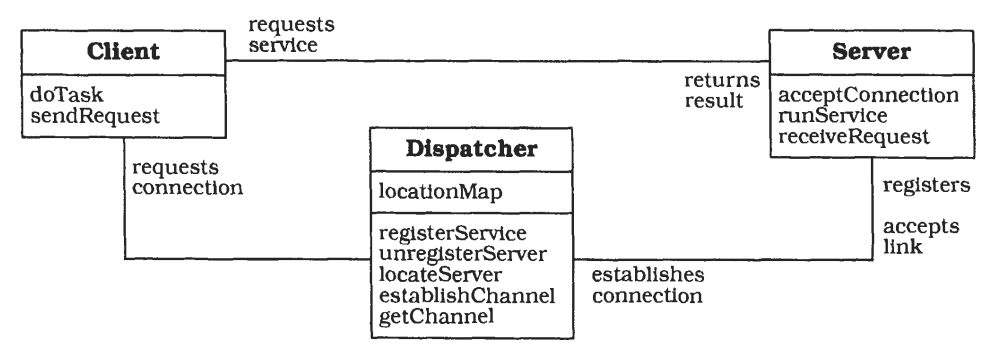
\includegraphics[width=0.8\textwidth]{figures/12-client-dispatcher-server-1.png}
	\caption{View Handler Komponenten}
\end{figure}

\section{Variants}


\section{Known Uses}


\section{Consequences}


\section{Relationships}


\section{Exam Questions}
\begin{itemize}
  	\item Behauptung:Dies ist eine Behauptung (Lösung: Lösung)
    \item Frage: Dies ist eine Frage? (Lösung)
\end{itemize}
